\chapter{Osterwalder's Business Model Ontology}
The goal for this project is to analyse the business potential of the exergame Cyberlab is going to develop. To do this, we have decided to use Osterwalder's Business Model Ontology. We analysed both Alexander Osterwalder's PhD thesis \cite{osterwalderthesis} and his textbook "Business Model Generation" \cite{osterwalder} and made our own synthesis of them. The thesis is a thoroughly description, while the book is easy to understand and on a more user friendly level. The foundation of our description lies in the textbook, with some details we found important from the thesis. In this way the description is well suited for our analysis.\\ \\
Osterwalder defines a business model like this: "A business model describes the rationale of how an organization creates, delivers, and captures values" \cite{osterwalder}. Osterwalder came up with a way to describe business models through nine building blocks. Going through these building blocks allow us to describe and think through the business model of any enterprise by covering four main areas of a business:  Product, Customer Interface, Infrastructure Management and Financial Aspects. The nine different building blocks are: Customer Segments, Value Propositions, Channels, Customer Relationships, Revenue Streams, Key Resources, Key Activities, Key Partnerships and Cost Structure \cite{osterwalder}. The nine business model elements are the core of the model, see Figure \ref{fig:TheBusinessModelCanvas}. 
In this chapter we will go through every of the nine building blocks in more detail. 

\begin{sidewaysfigure}
\centering
\scalebox{0.60}
{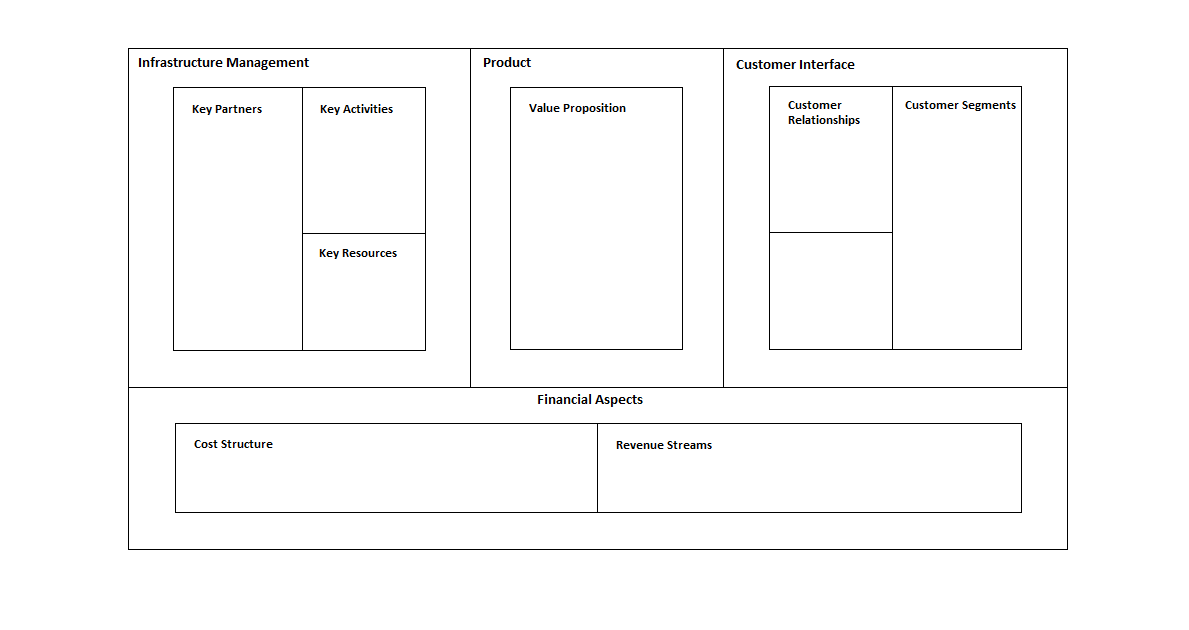
\includegraphics{osterwaldersbmmodified}}
\caption[The Business Model Canvas]{The Business Model Canvas [modified from \cite{osterwalder}]}
\label{fig:TheBusinessModelCanvas}
\end{sidewaysfigure}

\section{Product}
Product is what the company offers to its customer and how it differentiates itself from its competitors. This area covers the value proposition building block \cite{osterwalderthesis}.

\subsection{Value Proposition}
Osterwalder's definition is: "The Value Propositions Building Block describes the bundle of products and services that create value for a specific Customer Segment" \cite{osterwalder}. This is what the organization actually offers to their customer segment(s) and is suppose to satisfy the customers' needs. It might be different value propositions for the different customer segments. The values can be both quantitative and qualitative, meaning that the value can rely on for example price or on design. The value propositions have to be so good that the organization's defined customer segment(s) turn(s) to them over another company. It can be either something new, an improvement of already existing products or services, customized products and services, or simply just helping a customer to get a certain job done. Something to also consider is design and brand. These two aspects are more important in some type of products than other. It is also important to compare price levels with their competitors. A common way to satisfy the needs of the customer is to offer them the same value to a lower price. The firm can also keep-up with the market price, offer luxury goods to a higher price or simply offer a value proposition for free. For the latter, the model is based on another source of income, for example advertising. \\ \\
There are different ways of creating value for the customer. Reducing the costs will for most customers be experienced as valuable. Also reducing the risk when buying something, by for example offering them a one-year guarantee, is very satisfactory for customers. Other ways of creating value are to make products and services available for customers that did not have access to them before and to make products and services easier and more convenient to use. \cite{osterwalder}

\section{Customer Interface}
The customer interface covers everything that have to to with customers: who they are, what kind of relationship the firm has with them and how the firm reach out to them. The three building blocks covered by this area are thus: Customer Segments, Channels and Customer Relationships \cite{osterwalderthesis}.

\subsection{Customer Segments}
Osterwalder's definition is: "The Customer Segments Building Block defines the different groups of people or organizations an enterprise aims to reach and serve" \cite{osterwalder}. To make a good business, you have to understand who the business is meant to create value for, which is all about segmentation. It is important to carefully choose the most important customers and to focus on them and their needs. A business can have more than one customer segment, but they can not always serve all segments. Therefore a careful valuation has to be done to choose the organizations most important customer segment(s) \cite{osterwalder} \cite{osterwalderthesis}. \\ \\
A firm can deliver a value proposition to different types of customer segments. They can choose to not distinguish between customer segments and rather focus on the mass market; they can distinguish their customers into segments with slightly different needs or problems, or sharpen it even more by targeting a niche market with specialized customers. The firm can also serve unrelated customer segments or even independent customer segments \cite{osterwalder}.

\subsection{Channels}
Osterwalder's definition is: "The Channels Building Block describes how a company communicates with and reaches its Customer Segments to deliver a Value Proposition" \cite{osterwalder}. This is about finding the best and most cost-efficient way of reaching the right customers, at the right place and right time \cite{osterwalderthesis}. We distinguish between five channel phases, shown in Figure \ref{fig:ChannelPhases}. A channel should be studied over all these phases. It is important for an organization to think about how the customers want to be reached in all of these phases and how the channels can be integrated with the customers' routines. The ways the organization communicates with the customers is an important role in the customer experience. The value proposition can be delivered either directly, through for example sales force, or indirectly through intermediaries. They can also be delivered through owned channels, partner channels or a mix of both, see Figure  \ref{fig:ChannelTypes}
 \cite{osterwalderthesis}. \\ \\

\begin{figure}
\begin{center}
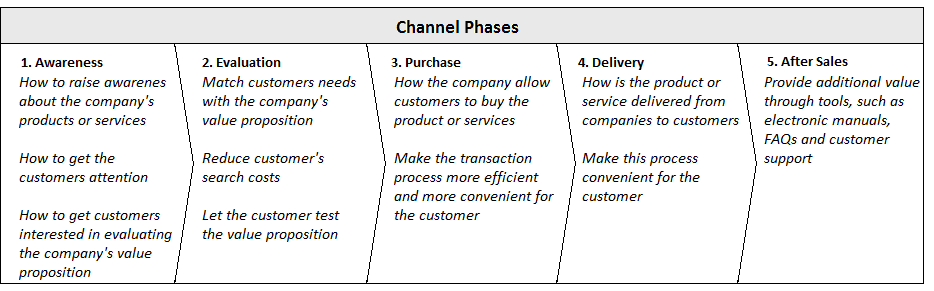
\includegraphics[angle=90,scale=0.6]{kjopskjede}
\caption[Channel Phases]{The 5 Channel Phases [modified from \cite{osterwalder}\cite{osterwalderthesis}]}
\label{fig:ChannelPhases}
\end{center}
\end{figure} 

\begin{figure}
\begin{center}
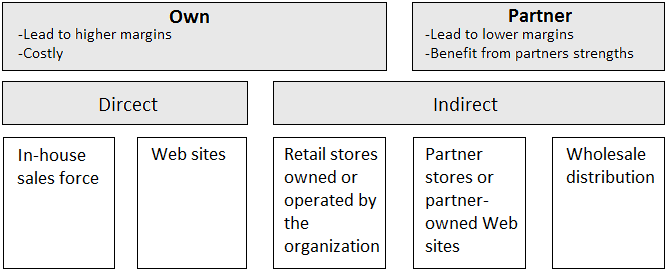
\includegraphics[scale=0.7]{channeltypes}
\caption[Channel Types]{Channel Types [modified from \cite{osterwalder}]}
\label{fig:ChannelTypes}
\end{center}
\end{figure} 

\newpage
\subsection{Customer Relationships}
Osterwalder's definition is: "The Customer Relationships Building Block describes the types of relationships a company establishes with specific Customer Segments" \cite{osterwalder}. The customer relationship is very important for the customers overall experience. This can range from personal assistance, where a real customer representative communicates with the customer, to a more automated service, where typically the customers help themselves,  to a more community based service that allows customer to exchange experiences with each other. For every type of customer segments defined, the organization has to keep in mind what kind of relationship the customer wishes to have. At the same time, the organization has to keep in mind how this relationship is integrated with the rest of their business model and how costly they are. The customer relationship is based on customer equity. There are three different customer equity goals: customer acquisition, customer retention and boosting sales (upselling) \cite{osterwalderthesis}.

\begin{itemize}
\renewcommand{\labelitemi}{$\bullet$}
\item \emph{Acquisition:} A company needs customers to do business. The customer acquisition is a very expensive affair and must be carefully managed and evaluated because the relationship developed with the customers will strongly influence the two next equity goals.
\item \emph{Retention:} After acquired customers, a goal should be to retain them. The customer acquisition is usually more expensive than customer retention. Because of this, ways to extend the duration of the relationship between the company and its (profitable) customers should be found. High switching costs is an element that can help retention. This means that the cost of ending the relationship and building a new one is so high that the customer does not want to switch.
\item \emph{Boosting sales (upselling):} This means adding on to the initial sale with additional products and services.
\end{itemize}

\section{Infrastructure Management}
Infrastructure management describes the company's capabilities and resources that are necessary to deliver the value proposition and maintain customer interface. This block also describes who provides and own the capabilities and resources, as well as who executes the activities and the relationship between them \cite{osterwalderthesis}.

\subsection{Key Resources}
Osterwalder's definition is: "The Key Resources Building Block describes the most important assets required to make a business model work" \cite{osterwalder}. This means all the resources you need to make all the 4 previous described building blocks work. The resources can be physical (e.g. buildings and machines), intellectual (e.g. brands, patents and copyrights), human (e.g. in an industry where knowledge is in particular important) and financial (e.g. cash). The company does not need to have all the resources within their organization; they can also be acquired from outside the company. A resource can be linked to one or more activities, described next.

\subsection{Key Activities}
Osterwalder’s definition is: "The Key Activities Building Block describes the most important things a company must do to make its business model work" \cite{osterwalder}. This means all the actions that have to be done to make all the 4 first building blocks described work and to generate profit. The main purpose of a company is the creation of value that customers are willing to pay for. This value is the outcome of a configuration of inside and outside activities and processes. Depending on what kind of company it is the configurations can by categorized as a \emph{Value Chain}, a \emph{Value Shop} or a \emph{Value Network}. Osterwalder distinguish between primary and support activities. Primary activities are involved in the creation of the value proposition and its marketing and delivery. Support activities are the underlying activities that have to be in place for the primary activities to take place (e.g. firm infrastructure, technology). All the three different types of configurations have different primary activities, as described in Figure \ref{fig:ValueChain}, \ref{fig:ValueShop} and \ref{fig:ValueNetwork} \cite{osterwalderthesis}:\\ \\
\emph{Value Chain:}
\begin{figure}[h]
\centering
\begin{center}
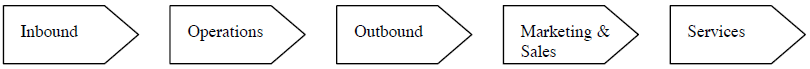
\includegraphics[scale=0.6]{valuechainnew}
\caption[Value Chain]{Value Chain (5 primary activities) \cite{osterwalderthesis}}
\label{fig:ValueChain}
\end{center}
\end{figure} \\ \\
A value chain describes how a firm creates value from taking an input, transforming it to the final product (refined output), distribute the product  to the customers and maintain the product (e.g. production and manufacturing). At each step there is added value. The main property for a value chain is being cost-efficient.
\newpage
\emph{Value Shop:}
\begin{figure}
\begin{center}
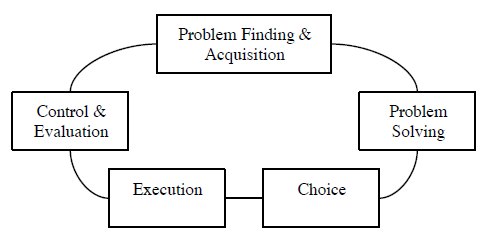
\includegraphics[scale=0.8]{valueshopnew}
\caption[Value Shop]{Value Shop (5 primary activities) \cite{osterwalderthesis}}
\label{fig:ValueShop}
\end{center}
\end{figure}
Value shop describes how a firm can create value for its customers by understanding their problem and finding a solution for it (e.g. consultancies and doctors). The main property of a value shop is rumour.  \\ \\
\emph{Value Network:}
This is about network effects, which means that the more people a network have the more value it gets. (e.g. banks and telecom operators). It involves getting potential customers to the network, establishing links between customers, billing them for the value received, and maintaining and running physical and information infrastructure so it is ready to serve customers requests. 
\begin{figure}
\begin{center}
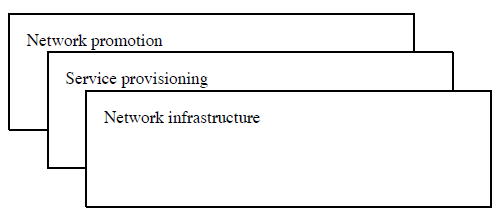
\includegraphics[scale=0.7]{valuenetworknew}
\caption[Value Network]{Value Network (3 primary activities) \cite{osterwalderthesis}}
\label{fig:ValueNetwork}
\end{center}
\end{figure}

\subsection{Key Partnerships}
Osterwalder’s definition is: “The Key Partnerships Building Block describes the network of suppliers and partners that make the business model work” \cite{osterwalder}. A company can not always do everything on their own. The motivation for creating partnerships can be divided in three \cite{osterwalder}: 
\\
1. \emph{Optimizing their business model:} Sometimes it is not profitable for a company to own all resources and do everything in-house. Cooperating with other firms can reduce costs and optimize the allocation of resources and activities. 
\\
2. \emph{Reduce risk:} In a very competitive market it can be safer to cooperate with the competitors in one area, even though they are competing in another.
\\
3. \emph{Acquire resources:} Usually it is not very profitable for a company to have all resources and to have the knowledge to do all the activities. Cooperating with other firms by buying/lending resources is often more profitable than having everything in-house. 

\section{Financial Aspects}
All of the other blocks just described influence this last area in the framework. Thus this area is an outcome of the rest of the business model configuration and covers the Revenue Streams and Cost Structure elements. \cite{osterwalderthesis}

\subsection{Revenue Streams}
Osterwalder’s definition is: "The Revenue Streams Building Block represents the cash a company generates from each Customer Segment" \cite{osterwalder}. This is where the company earns money and generate profit. It is important to keep in mind what the customers are willing to pay, as well as what they are currently paying. A firm can have one or more revenue streams where each revenue stream can have different pricing mechanisms.  Possible ways to generate revenue streams are listed in Table \ref{tab:revenue}  \\ \\ 
The pricing mechanism chosen is very important and can make a huge difference on how much revenue that is generated. Osterwalder distinguish between two types of pricing mechanisms: fixed and dynamic pricing, where fixed pricing means that the prices are based on static variables, while dynamic means that prices changes with market conditions \cite{osterwalder}.

\begin{table}
\centering
     \caption[Different ways to generate revenue streams]{Different ways to generate revenue streams}
    \begin{tabular}{|l|l|}
  
        \hline
       \textbf{Ways to generate revenue} & \textbf{Example}  \\ \hline
       \emph{Asset sale} & Selling a car \\ \hline
       \emph{Usage fee} & Customer pays telecom operator for minutes \\ & spend on the phone \\ \hline
	 	\emph{Subscription fee} & Users of Spotify pay a monthly fee to access \\ & Spotify Premium \\ \hline
	   \emph{Renting} & Renting a car for the weekend \\ \hline
	   \emph{Licensing}	& Companies have to pay a license fee to get \\ & access to patented technology  \\ \hline
	   \emph{Brokerage fee}	& A seller that earns a commission each time \\ & he sells a product  \\ \hline
	   \emph{Advertising} & A newspaper takes a fee from companies \\ & who wants to promote their product \\ &in the newspaper \\ \hline
    \end{tabular}
    \label{tab:revenue}
\end{table}

\subsection{Cost Structure}
Osterwalder’s definition is: “The Cost Structure describes all costs incurred to operate a business model” \cite{osterwalder}. The costs in the business model come from Key Resources, Key Activities and Key Partnerships. The book \cite{osterwalder} defines two cost structures: cost-driven business model, which focus on minimizing costs, and value-driven business model, which are focussing on value creation by for example making personalized services. Both cost structures can have different characteristics, shown in Table \ref{tab:cost} \cite{osterwalder}. \\ \\

\begin{table}
\centering
 \caption[Characteristics of cost structures]{Characteristics of cost structures}
    \begin{tabular}{|l|l|}
        \hline
        \textbf{Type} & \textbf{Description} \\ \hline
       Fixed costs & Costs stay the same regardless of the volume  \\ \hline
       Variable costs & Costs depend on volume \\ \hline
       Economies of scale & Less cost as output increases \\ \hline
	   Economies of scope & Less cost due to larger scope of operations \\ \hline
    \end{tabular}
    \label{tab:cost}
\end{table}

Based on this business model framework, we will analyse the potential of the game. To gather information we have performed interviews with physiotherapists to find out if they are the right customer segment or not. We have used the nine building blocks as a basis for the questions asked in the interviews.
